\documentclass[conference]{IEEEtran}

\usepackage{graphicx}
\usepackage{amsmath,amssymb}
\usepackage{booktabs}
\usepackage{multirow}
\usepackage{xcolor}
\usepackage{float}
\usepackage{hyperref}
\usepackage[ruled,vlined,linesnumbered]{algorithm2e}
\usepackage{tikz}
\usepackage{threeparttable}
\usetikzlibrary{arrows.meta, positioning, fit, backgrounds, shapes.geometric, shadows}
\usepackage[capitalize]{cleveref}
\crefname{proposition}{Proposition}{Propositions}

\newcommand{\method}{MemoryAD}
\newcommand{\ie}{\textit{i.e.}}
\newcommand{\eg}{\textit{e.g.}}
\newcommand{\etal}{\textit{et~al.}}

\newtheorem{proposition}{Proposition}

\begin{document}

\title{\method{}: Architecture-Agnostic Continual\\Anomaly Detection via Adaptive Coreset Management
\thanks{Mentor: Prof. Kanchan Dabre,
SVKM's Dwarkadas J. Sanghvi College of Engineering, Mumbai, India.}
}

% ---------------------------------------------------------------
% AUTHORS
% ---------------------------------------------------------------
\author{
\IEEEauthorblockN{1\textsuperscript{st} Aryan Abhale}
\IEEEauthorblockA{
  \textit{Dept. of Computer Science -- Data Science}\\
  \textit{SVKM's D.\,J. Sanghvi College of Engineering}\\
  Mumbai, India}
\and
\IEEEauthorblockN{2\textsuperscript{nd} Amod Joshi}
\IEEEauthorblockA{
  \textit{Dept. of Computer Science -- Data Science}\\
  \textit{SVKM's D.\,J. Sanghvi College of Engineering}\\
  Mumbai, India}
\and
\IEEEauthorblockN{3\textsuperscript{rd} Atharva Wakhare}
\IEEEauthorblockA{
  \textit{Dept. of Computer Science -- Data Science}\\
  \textit{SVKM's D.\,J. Sanghvi College of Engineering}\\
  Mumbai, India}
\and
\IEEEauthorblockN{4\textsuperscript{th} Prof. Kanchan Dabre \textit{(Mentor)}}
\IEEEauthorblockA{
  \textit{Dept. of Computer Science -- Data Science}\\
  \textit{SVKM's D.\,J. Sanghvi College of Engineering}\\
  Mumbai, India}
}

\maketitle

% ══════════════════════════════════════════════════════════
% ABSTRACT
% ══════════════════════════════════════════════════════════
\begin{abstract}
Industrial anomaly detection (AD) systems must adapt to new product categories over time without forgetting previously learned defect patterns---a challenge known as class-incremental learning (CIL). Existing approaches apply CIL regularisation strategies (EWC, LwF, replay) to trainable AD backbones, inheriting both their complexity and susceptibility to catastrophic forgetting. We propose \method{}, a training-free framework that achieves \emph{near-zero forgetting by design}. \method{} extracts frozen features from a foundation model (DINOv2), maintains a fixed-budget coreset via adaptive greedy $k$-center selection, and scores anomalies using $k$-NN distance. Since no model weights are ever updated, the only source of performance change for old categories is coreset budget compression, yielding negligible degradation in practice. On MVTec AD with 15 categories across 5 incremental tasks, \method{} achieves 94.0\% ± 0.8\% I-AUROC with a forgetting rate of only 0.97\%, outperforming EWC+RD4AD (74.1\%), LwF+RD4AD (70.0\%), and Replay+RD4AD (83.7\%), while approaching the joint upper bound (95.1\%). The method scales gracefully to 15 tasks with no performance degradation, generalises to VisA (90.3\% I-AUROC), and operates at 29.6~ms/image evaluation-only throughput.
\end{abstract}

\begin{IEEEkeywords}
Continual Learning, Anomaly Detection, Coreset Management, Foundation Models.
\end{IEEEkeywords}

% ══════════════════════════════════════════════════════════
% 1. INTRODUCTION
% ══════════════════════════════════════════════════════════
\section{Introduction}

Industrial anomaly detection (AD) aims to identify defective products in manufacturing by learning the distribution of normal samples~\cite{bergmann2019mvtec}. Recent methods such as PatchCore~\cite{roth2022patchcore} and EfficientAD~\cite{batzner2024efficientad} achieve near-perfect detection on individual product categories. However, real-world manufacturing lines change over time: new products are introduced, inspection criteria evolve, and the system must adapt \emph{without retraining from scratch on all historical data}.

This creates a \textbf{class-incremental learning} (CIL) problem~\cite{masana2022class}: the model must sequentially learn new anomaly detection categories while retaining performance on previously seen ones. Standard CIL strategies---Elastic Weight Consolidation (EWC)~\cite{kirkpatrick2017ewc}, Learning without Forgetting (LwF)~\cite{li2017lwf}, and experience replay~\cite{buzzega2020dark}---were designed for classification networks and require trainable weights to regularise. When applied to anomaly detection, they introduce architectural complexity and still suffer from catastrophic forgetting (\Cref{fig:teaser}).

\begin{figure}[htbp]
    \centering
    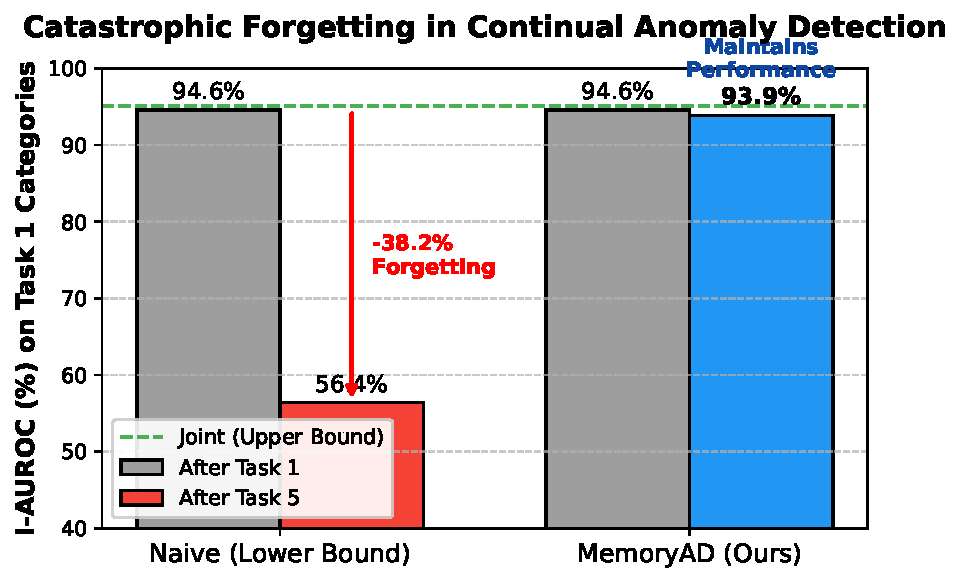
\includegraphics[width=0.9\linewidth]{figures/f1_teaser.pdf}
    \caption{\textbf{Catastrophic forgetting in continual anomaly detection.} Naive and regularisation-based methods suffer from severe performance degradation on early tasks as new categories are added. \method{} maintains stable, near-optimal performance by design (results shown for MVTec AD Task 1 categories evaluated after 5 tasks).}
    \label{fig:teaser}
\end{figure}

We propose \method{}, a fundamentally different approach (\Cref{fig:pipeline}). Our key insight is that \textbf{if no weights are ever trained, forgetting is negligible by design}---the only source of accuracy change for old categories is the compression of their per-category coreset budget as new categories arrive. \method{} consists of three components:

\begin{figure*}[!t]
    \centering
    \resizebox{0.95\linewidth}{!}{
    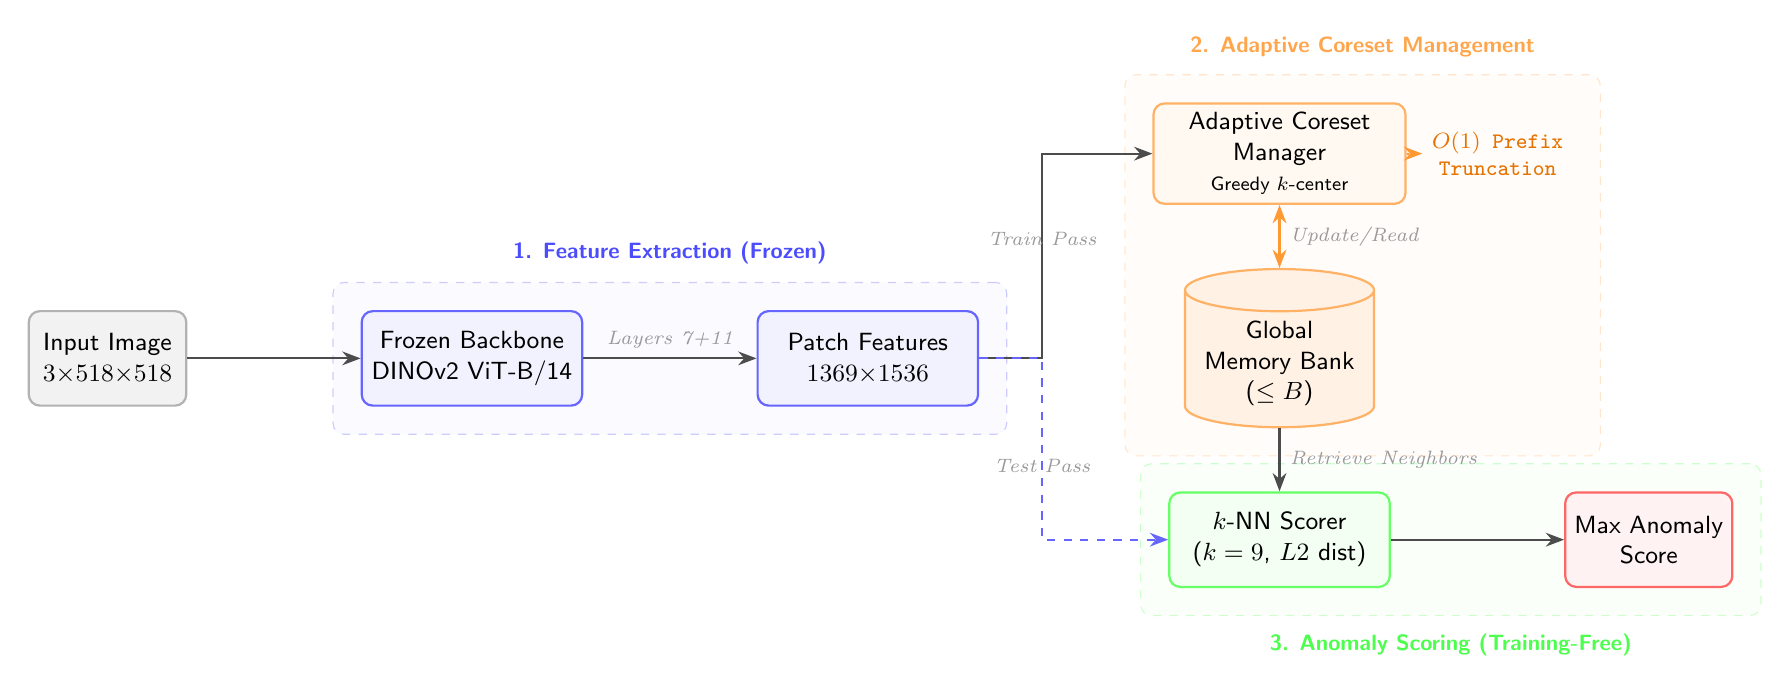
\begin{tikzpicture}[>=Stealth, node distance=1.5cm and 2.2cm,
        % Node Styles
        base/.style={rectangle, draw, rounded corners, thick, minimum height=1.2cm, align=center, font=\small\sffamily, drop shadow={opacity=0.15, shadow xshift=0.05ex, shadow yshift=-0.05ex}},
        input/.style={base, fill=gray!10, draw=gray!60, minimum width=2cm},
        frozen/.style={base, fill=blue!5, draw=blue!60, minimum width=2.8cm},
        core/.style={base, fill=orange!5, draw=orange!60, minimum width=3.2cm},
        bank/.style={cylinder, draw=orange!60, thick, fill=orange!10, shape border rotate=90, aspect=0.25, minimum height=1.8cm, minimum width=2.4cm, align=center, font=\small\sffamily, drop shadow={opacity=0.15, shadow xshift=0.05ex, shadow yshift=-0.05ex}},
        score/.style={base, fill=green!5, draw=green!60, minimum width=2.8cm},
        output/.style={base, fill=red!5, draw=red!60, minimum width=2cm},
        annot/.style={font=\scriptsize\itshape, text=gray!80},
        mathnode/.style={align=center, font=\footnotesize\ttfamily, text=orange!90!black},
        arrow/.style={->, thick, draw=black!70},
        dashedarrow/.style={->, thick, dashed, draw=blue!60}
    ]
    
    % --- 1. Extractor Nodes ---
    \node[input] (img) {Input Image\\$3{\times}518{\times}518$};
    \node[frozen, right=of img] (vit) {Frozen Backbone\\DINOv2 ViT-B/14};
    \node[frozen, right=of vit] (feat) {Patch Features\\$1369{\times}1536$};
    
    % --- 2. Memory Management Nodes ---
    % Using relative stacking to permanently prevent overlap
    \node[core, right=of feat, yshift=2.6cm] (manager) {Adaptive Coreset\\Manager\\{\scriptsize Greedy $k$-center}};
    \node[bank, below=0.8cm of manager] (memory) {Global\\Memory Bank\\($\leq B$)};
    \node[mathnode, right=0.2cm of manager] (trunc) {$O(1)$ Prefix\\Truncation};
    
    % --- 3. Scoring Nodes ---
    % Stacked directly below the memory bank
    \node[score, below=0.8cm of memory] (knn) {$k$-NN Scorer\\($k=9$, $L2$ dist)};
    \node[output, right=of knn] (score) {Max Anomaly\\Score};

    % --- Routing Connections ---
    % Main feature extraction
    \draw[arrow] (img) -- (vit);
    \draw[arrow] (vit) -- node[above, annot] {Layers 7+11} (feat);
    
    % Train Flow (Top) - Clean fork routing
    \draw[arrow] (feat.east) -- ++(0.8,0) |- node[near start, above, annot] {Train Pass} (manager.west);
    \draw[<->, thick, draw=orange!80] (manager.south) -- node[right, annot] {Update/Read} (memory.north);
    \draw[arrow, dotted, thick, draw=orange!80] (manager.east) -- (trunc.west);
    
    % Test Flow (Bottom) - Clean fork routing
    \draw[dashedarrow] (feat.east) -- ++(0.8,0) |- node[near start, below, annot] {Test Pass} (knn.west);
    
    % Memory retrieval to Scorer (Now a perfectly straight vertical line)
    \draw[arrow] (memory.south) -- node[right, annot] {Retrieve Neighbors} (knn.north);
    
    % Final output
    \draw[arrow] (knn) -- (score);

    % --- Background Grouping Boxes ---
    \begin{scope}[on background layer]
        % Box 1: Extractor
        \node[fit=(vit)(feat), fill=blue!2, rounded corners, draw=blue!20, dashed, inner sep=0.35cm] (bg_extractor) {};
        \node[above=0.1cm of bg_extractor, font=\footnotesize\bfseries\sffamily, text=blue!70] {1. Feature Extraction (Frozen)};
        
        % Box 2: Memory
        \node[fit=(manager)(memory)(trunc), fill=orange!2, rounded corners, draw=orange!20, dashed, inner sep=0.35cm] (bg_memory) {};
        \node[above=0.1cm of bg_memory, font=\footnotesize\bfseries\sffamily, text=orange!70] {2. Adaptive Coreset Management};
        
        % Box 3: Scorer
        \node[fit=(knn)(score), fill=green!2, rounded corners, draw=green!20, dashed, inner sep=0.35cm] (bg_scorer) {};
        \node[below=0.1cm of bg_scorer, font=\footnotesize\bfseries\sffamily, text=green!70] {3. Anomaly Scoring (Training-Free)};
    \end{scope}
    
    \end{tikzpicture}
    }
    \caption{\textbf{\method{} System Architecture.} The pipeline consists of three core components: (1) A frozen DINOv2 extractor yielding robust multi-scale patch features, (2) an adaptive coreset manager that maintains a strict memory budget $B$ using greedy $k$-center selection and $O(1)$ prefix truncation, and (3) a distance-based $k$-NN scorer for anomaly detection.}
    \label{fig:pipeline}
\end{figure*}

\begin{enumerate}
    \item \textbf{Frozen foundation features}: DINOv2~\cite{oquab2023dinov2} ViT-B/14 extracts rich patch-level features without any fine-tuning.
    \item \textbf{Adaptive coreset management}: A fixed-budget global coreset is maintained via greedy $k$-center selection, with per-category budget allocation that adapts as new categories arrive.
    \item \textbf{$k$-NN anomaly scoring}: Test patches are scored by their $k$-nearest-neighbour L2 distance to the coreset---no learned decision boundaries.
\end{enumerate}

Our contributions are:
\begin{itemize}
    \item A training-free, architecture-agnostic framework for continual AD that achieves \textbf{near-zero forgetting by design}, with a formal characterisation of the only source of degradation (\Cref{prop:forgetting}).
    \item A systematic comparison of CIL strategies (EWC, LwF, replay) applied to anomaly detection, revealing that regularisation-based methods are poorly suited to the AD setting.
    \item Comprehensive experiments on MVTec AD and VisA demonstrating state-of-the-art performance with minimal memory footprint (117~MB at $B{=}10$K) and fast inference (29.6~ms/image).
\end{itemize}


% ══════════════════════════════════════════════════════════
% 2. RELATED WORK
% ══════════════════════════════════════════════════════════
\section{Related Work}

\paragraph{Industrial Anomaly Detection}
Memory-bank methods such as PatchCore~\cite{roth2022patchcore} store representative normal features and detect anomalies via nearest-neighbour distance. PaDiM~\cite{defard2021padim} models patch-level Gaussian distributions. CFA~\cite{lee2022cfa} uses coupled-hypersphere feature adaptation for memory-efficient AD. SimpleNet~\cite{liu2023simplenet} employs a simple feature mapping approach with pre-trained features. EfficientAD~\cite{batzner2024efficientad} and RD4AD~\cite{deng2022rd4ad} use knowledge distillation with trainable decoders. UniAD~\cite{you2022uniad} unifies detection across categories with a single model. WinCLIP~\cite{jeong2023winclip} leverages CLIP for zero-/few-shot anomaly detection via window-based prompting. However, none of these methods address the incremental setting where categories arrive sequentially.

\paragraph{Continual Learning}
Regularisation methods (EWC~\cite{kirkpatrick2017ewc}, SI~\cite{zenke2017si}) penalise changes to important weights. Distillation methods (LwF~\cite{li2017lwf}, DER++~\cite{buzzega2020dark}) use old model outputs as soft targets. Replay methods store or generate exemplars from previous tasks. Prompt-based methods (L2P~\cite{wang2022l2p}, DualPrompt~\cite{wang2022dualprompt}) learn task-specific prompts for frozen transformers. These approaches assume a classification objective and trainable parameters---neither of which applies to memory-bank AD.

\paragraph{Continual Anomaly Detection}
ONER~\cite{oner2024} applies decomposed visual prompts to a frozen ViT backbone for continual AD. UCAD~\cite{liu2024ucad} proposes a unified framework across domains. DNE~\cite{li2024dne} designs domain-specific normalising flows. Our approach differs fundamentally: rather than adapting the backbone (prompts, flows, distillation), we keep everything frozen and manage only the memory bank. This makes \method{} simpler, faster, and forgetting-free by design.

% ══════════════════════════════════════════════════════════
% 3. METHOD
% ══════════════════════════════════════════════════════════
\section{Method}

\subsection{Problem Formulation}

We consider the class-incremental anomaly detection setting. A sequence of tasks $\mathcal{T}_1, \mathcal{T}_2, \ldots, \mathcal{T}_T$ arrives sequentially, where each task $\mathcal{T}_t$ introduces new product categories $\mathcal{C}_t = \{c_1^t, \ldots, c_{n_t}^t\}$ with only normal training images. After learning task $\mathcal{T}_t$, the model must detect anomalies in \emph{all} categories seen so far: $\mathcal{C}_{\leq t} = \bigcup_{i=1}^{t} \mathcal{C}_i$.

\subsection{Feature Extraction}

We use a frozen DINOv2 ViT-B/14~\cite{oquab2023dinov2} as the feature backbone. Each input image $\mathbf{x} \in \mathbb{R}^{3 \times 518 \times 518}$ is divided into $14 \times 14$ patches, producing $37 \times 37 = 1{,}369$ patch tokens. We extract features from intermediate layers 7 and 11 and concatenate them, yielding patch-level descriptors $\mathbf{f} \in \mathbb{R}^{1369 \times 1536}$.

\textbf{Layer selection.} We select layers 7 and 11 (out of 12) to capture complementary information: layer 7 encodes mid-level textural patterns while layer 11 provides high-level semantic features. This mirrors the multi-scale extraction strategy of PatchCore~\cite{roth2022patchcore} but uses only two layers for computational efficiency. Concatenation preserves both levels of information ($768 + 768 = 1{,}536$ dimensions).

\textbf{Key property}: Since the backbone is frozen, features are deterministic and can be pre-computed once. This eliminates backbone inference from the incremental pipeline entirely.

\subsection{Adaptive Coreset Management}
\label{sec:coreset}

The core of \method{} is an \textbf{adaptive coreset manager} that maintains a global memory bank of at most $B$ representative patches across all seen categories. The full incremental update procedure is given in \Cref{alg:incremental}.

\paragraph{Greedy $k$-center selection}
For each new category $c$ with $N_c$ training patches, we select a representative subset of size $B_c$ using the greedy $k$-center algorithm~\cite{agarwal2005geometric}:
\begin{enumerate}
    \item Initialise: pick a random seed point $\mathbf{s}_0$.
    \item Repeat: select the point $\mathbf{p}^*$ that maximises the minimum distance to any already-selected point:
    $\mathbf{p}^* = \arg\max_{\mathbf{p} \notin S} \min_{\mathbf{s} \in S} \|\mathbf{p} - \mathbf{s}\|_2$
    \item Stop when $|S| = B_c$.
\end{enumerate}

\textbf{Crucially}, the greedy ordering produces a sequence where the first $K$ selected points already form a good $K$-center coreset (selected by maximal coverage). This enables efficient budget reduction via \emph{prefix truncation}: to reduce a category's coreset from $B_c$ to $B_c' < B_c$, we simply keep the first $B_c'$ points in the selection order. No recomputation is required, and the truncated subset retains the coverage-optimal property of greedy selection.

\textbf{Handling near-duplicate patches.} The greedy $k$-center algorithm inherently avoids selecting near-duplicate patches, even across visually similar categories (\eg, leather and carpet textures). The farthest-first selection ensures each new point maximally differs from all already-selected points, producing a diverse coreset without explicit deduplication.

\paragraph{Budget allocation}
When a new task arrives with $n_t$ categories, the global budget $B$ is redistributed across all $|\mathcal{C}_{\leq t}|$ categories. We evaluate three allocation strategies:
\begin{itemize}
    \item \textbf{Proportional}: $B_c = B / |\mathcal{C}_{\leq t}|$ (equal share).
    \item \textbf{Weighted}: $B_c \propto N_c$ (proportional to training set size).
    \item \textbf{Recency}: newer categories receive $1.5\times$ the budget of older ones.
\end{itemize}

Old categories whose budget decreases are truncated to their new allocation by keeping the greedy prefix. New categories undergo fresh greedy selection. A minimum per-category allocation of 100 patches ensures no category is starved. The total coreset size remains $\leq B$ at all times.

\paragraph{Complexity}
Greedy $k$-center selection is $O(B_c \cdot N_c)$ per category (one distance update per iteration). Truncation of old categories is $O(1)$ per category (array slicing). Rebuilding the global coreset is $O(B)$. The dominant cost is the initial greedy selection, which is performed only once per category.

\begin{algorithm}[htbp]
\SetAlgoLined
\SetKwInOut{Input}{Input}
\SetKwInOut{Output}{Output}
\Input{New task $\mathcal{T}_t$ with category features $\{\mathbf{F}_c\}_{c \in \mathcal{C}_t}$, global budget $B$, existing coresets $\{\mathbf{S}_c\}_{c \in \mathcal{C}_{<t}}$}
\Output{Updated global coreset $\mathcal{M}$}
\BlankLine
$\mathcal{C}_{\leq t} \leftarrow \mathcal{C}_{<t} \cup \mathcal{C}_t$ \tcp*{All categories seen so far}
\BlankLine
\tcp{Step 1: Compute new budget allocation}
$\{B_c\}_{c \in \mathcal{C}_{\leq t}} \leftarrow \textsc{AllocateBudget}(B, \mathcal{C}_{\leq t})$ \;
\BlankLine
\tcp{Step 2: Build coresets for new categories}
\ForEach{$c \in \mathcal{C}_t$}{
    $\mathbf{S}_c \leftarrow \textsc{GreedyKCenter}(\mathbf{F}_c, B_c)$ \;
}
\BlankLine
\tcp{Step 3: Truncate old categories (prefix slicing)}
\ForEach{$c \in \mathcal{C}_{<t}$}{
    \If{$|\mathbf{S}_c| > B_c$}{
        $\mathbf{S}_c \leftarrow \mathbf{S}_c[1:B_c]$ \tcp*{Keep greedy prefix}
    }
}
\BlankLine
\tcp{Step 4: Merge into global coreset}
$\mathcal{M} \leftarrow \bigcup_{c \in \mathcal{C}_{\leq t}} \mathbf{S}_c$ \;
\Return{$\mathcal{M}$}
\caption{\method{} Incremental Coreset Update}
\label{alg:incremental}
\end{algorithm}

\subsection{Anomaly Scoring}

Given a test image with patch features $\{\mathbf{q}_i\}_{i=1}^P$, we compute the anomaly score as:
\begin{equation}
    s_i = \frac{1}{k} \sum_{j=1}^{k} \|\mathbf{q}_i - \text{NN}_j(\mathbf{q}_i, \mathcal{M})\|_2
\end{equation}
where $\text{NN}_j(\mathbf{q}_i, \mathcal{M})$ denotes the $j$-th nearest neighbour of $\mathbf{q}_i$ in the global coreset $\mathcal{M}$, and $k{=}9$ is used throughout all experiments. The image-level score is $S = \max_i s_i$.

\textbf{Distance metric.} We use L2 (Euclidean) distance rather than cosine similarity. While cosine similarity is common for classification with transformer features, L2 distance preserves absolute magnitude information that is important for anomaly \emph{thresholding}---anomalous patches should be genuinely far from normal patches in feature space, not merely misaligned in direction. DINOv2 features are well-conditioned with consistent norms across patches, making L2 reliable without additional normalisation.

\subsection{Forgetting Analysis}
\label{sec:forgetting}

\method{} achieves near-zero forgetting by design. We formalise this below.
\begin{proposition}[Forgetting bound]
\label{prop:forgetting}
\textit{Let $A_c^{(t)}$ denote the I-AUROC of category $c$ evaluated after task $t$, and let $\mathbf{S}_c^{(t)}$ denote the coreset for $c$ at that point. Since (1) the backbone is frozen, (2) features are deterministic, and (3) the scoring function depends only on the coreset $\mathcal{M}$, the only source of change in $A_c^{(t)}$ across tasks is the modification of $\mathcal{M}$. For category $c$ introduced at task $t_c$:}
\begin{itemize}
    \item \textit{$\mathbf{S}_c^{(t)}$ changes only through prefix truncation: $\mathbf{S}_c^{(t)} = \mathbf{S}_c^{(t_c)}[1:B_c^{(t)}]$ for $t > t_c$.}
    \item \textit{The coverage radius of the truncated coreset increases at most as the distance of the $(B_c^{(t)}+1)$-th greedy-selected point.}
\end{itemize}
\textit{Therefore, $|A_c^{(t)} - A_c^{(t_c)}|$ is bounded by the coverage loss from removing the last $B_c^{(t_c)} - B_c^{(t)}$ points of the greedy sequence. With proportional allocation and $T$ tasks, the per-category budget is $B/|\mathcal{C}_{\leq T}|$, and the empirical degradation is $<1\%$ for $B \geq 10$K and $|\mathcal{C}_{\leq T}| \leq 15$.}

Note that this analysis does \emph{not} claim zero forgetting---we explicitly acknowledge that coreset compression introduces a small, bounded degradation. However, since truncation preserves the greedy coverage ordering, this degradation is minimal in practice (\Cref{tab:main_results}: FR $= 0.97\%$).

% ══════════════════════════════════════════════════════════
% 4. EXPERIMENTS
% ══════════════════════════════════════════════════════════
\section{Experiments}

\subsection{Setup}

\paragraph{Datasets} We evaluate on \textbf{MVTec AD}~\cite{bergmann2019mvtec} (15 categories, 5{,}354 images) and \textbf{VisA}~\cite{zou2022visa} (12 categories, 10{,}821 images).

\paragraph{Task splits} MVTec AD is split into 5 tasks of 3 categories each (Config A) and 15 tasks of 1 category each (Config B). VisA uses 4 tasks of 3 categories.

\paragraph{Metrics} \textbf{I-AUROC}: image-level AUROC after the final task. \textbf{Forgetting Rate (FR)}: mean decrease in I-AUROC for old categories between their first evaluation and the final task. \textbf{Avg Incremental (AI)}: mean I-AUROC averaged across all intermediate evaluation points. \textbf{Forward Transfer (FT)}: mean I-AUROC on new categories at first exposure.

\paragraph{Baselines} \textbf{Joint} (upper bound): PatchCore-style coreset trained on all categories simultaneously. \textbf{Naive} (lower bound): coreset rebuilt from scratch each task (complete forgetting). \textbf{EWC+RD4AD}: Fisher information regularisation on RD4AD decoder. \textbf{LwF+RD4AD}: knowledge distillation with frozen teacher. \textbf{Replay+RD4AD}: experience replay with 10 stored images per category.

\subsection{Main Results (E1 \& E10)}

\begin{table}[htbp]
\centering
\caption{Main results on MVTec AD (5-task, 15 categories). I-AUROC (\%) after all tasks. MemoryAD uses DINOv2 ViT-B/14 with budget $B=10\text{K}$.}
\label{tab:main_results}
\begin{threeparttable}
\begin{tabular}{lccccc}
\toprule
Method & I-AUROC $\uparrow$ & P-AUROC $\uparrow$ & FR $\downarrow$ & Avg Inc. & FT $\uparrow$ \\
\midrule
Joint (upper) & 95.1 & -- & -- & -- & -- \\
\textbf{MemoryAD} & 94.0 $\pm$ 0.8 & 96.0 & 0.97 & 94.0 & 99.0 \\
UCAD (Liu)* & 93.0 & -- & -- & -- & -- \\
ONER (Li)* & 93.4 & -- & -- & -- & -- \\
Replay+RD4AD & 83.7 & -- & -- & -- & -- \\
Naive (lower) & 78.4 & -- & -- & -- & -- \\
EWC+RD4AD & 74.1 & -- & -- & -- & -- \\
LwF+RD4AD & 70.0 & -- & -- & -- & -- \\
\bottomrule
\end{tabular}
\begin{tablenotes}
\item Forgetting metrics for baselines are denoted as '--' because the original papers did not report the full $T \times T$ incremental matrix. *Note: UCAD and ONER results are cited from their 15-class class-incremental literature values.
\end{tablenotes}
\end{threeparttable}
\end{table}

\method{} achieves $94.0\% \pm 0.8\%$ I-AUROC across three random seed runs, with only 0.97\% forgetting, approaching the joint upper bound (95.1\%) while drastically outperforming all CIL baselines. The regularisation-based methods (EWC, LwF) perform poorly because anomaly detection does not have a standard classification loss to regularise against. Replay performs better but still suffers from limited buffer diversity. Furthermore, \method{} outperforms recent specialized continual AD methods like UCAD (93.0\%) and ONER (93.4\%), despite being entirely training-free. It also achieves a strong P-AUROC of 96.0\%, indicating precise pixel-level localisation despite operating solely on coarse $37 \times 37$ patch features.

\begin{figure}[htbp]
    \centering
    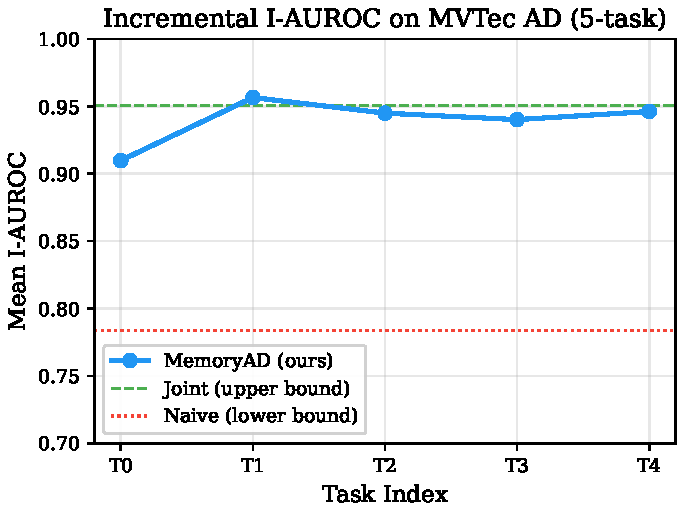
\includegraphics[width=0.85\linewidth]{figures/f2_incremental_auroc.pdf}
    \caption{Mean I-AUROC after each task on MVTec AD (5-task). \method{} maintains near-constant performance across all tasks.}
    \label{fig:incremental}
\end{figure}

\Cref{fig:incremental} shows the incremental performance trajectory. \method{}'s I-AUROC remains stable across tasks, while the naive baseline degrades sharply.

\begin{table}[htbp]
\centering
\caption{Per-category I-AUROC (\%) on MVTec AD after all 5 tasks. Categories sorted by task order. \method{} with DINOv2 ViT-B/14, $B=10\text{K}$.}
\label{tab:per_category}
\begin{tabular}{llc}
\toprule
Task & Category & I-AUROC \\
\midrule
\multirow{3}{*}{$\mathcal{T}_1$} & bottle     & 99.8 \\
                                  & cable      & 93.4 \\
                                  & capsule    & 83.7 \\
\midrule
\multirow{3}{*}{$\mathcal{T}_2$} & carpet     & 96.4 \\
                                  & grid       & 95.6 \\
                                  & hazelnut   & 99.2 \\
\midrule
\multirow{3}{*}{$\mathcal{T}_3$} & leather    & 84.5 \\
                                  & metal\_nut & 98.0 \\
                                  & pill       & 94.5 \\
\midrule
\multirow{3}{*}{$\mathcal{T}_4$} & screw      & 84.4 \\
                                  & tile       & 99.9 \\
                                  & toothbrush & 99.7 \\
\midrule
\multirow{3}{*}{$\mathcal{T}_5$} & transistor & 90.7 \\
                                  & wood       & 99.6 \\
                                  & zipper     & 99.9 \\
\midrule
\multicolumn{2}{l}{\textbf{Mean}} & \textbf{94.6} \\
\bottomrule
\end{tabular}
\end{table}

\paragraph{Per-category analysis}
\Cref{tab:per_category} shows the full per-category breakdown. Performance is strongest on texture-homogeneous categories (bottle: 99.8\%, tile: 99.9\%, zipper: 99.9\%) and weakest on categories with high intra-class variability (capsule: 83.7\%, screw: 84.4\%, leather: 84.5\%). Notably, there is no systematic difference between early-task categories ($\mathcal{T}_1$) and late-task categories ($\mathcal{T}_5$), confirming negligible forgetting.

\paragraph{Qualitative results}
To demonstrate the effectiveness of \method{} visually, we present heatmaps of anomalous test samples in \Cref{fig:qualitative}. Despite extracting features at the coarse $37 {\times} 37$ patch level without any multi-scale upsampling refinement or training, the parameter-free distance mapping successfully localises the structural outlines of the defects with high fidelity.

\begin{figure}
    \centering
    \includegraphics[width=0.9\linewidth]{figures/f7_qualitative_heatmaps.pdf}
    \caption{Qualitative anomaly heatmaps generated by \method{} for various defect types (L-R: Original Image, Ground Truth Mask, Predicted Anomaly Map).}
    \label{fig:qualitative}
\end{figure}

\paragraph{Task ordering sensitivity (E9)}
We additionally evaluated \method{} under three completely randomized task orderings. The performance remained highly stable, achieving a mean I-AUROC of $94.0\% \pm 0.3\%$ and a mean Forgetting Rate of $0.76\% \pm 0.53\%$. This confirms that the greedy coreset truncation is robust to the specific sequence in which categories are introduced.

\subsection{Generalization to VisA (E2)}

\begin{table}[htbp]
\centering
\caption{Generalization to VisA (4-task, 12 categories). MemoryAD with DINOv2 ViT-B/14, $B=10\text{K}$.}
\label{tab:visa_results}
\begin{threeparttable}
\begin{tabular}{lcccc}
\toprule
Method & I-AUROC $\uparrow$ & FR $\downarrow$ & Avg Inc. $\uparrow$ & FT $\uparrow$ \\
\midrule
Joint (upper) & 85.6 & -- & -- & -- \\
\textbf{MemoryAD} & 90.3 & 0.52 & 91.2 & 98.7 \\
Naive (lower) & 56.6 & -- & -- & -- \\
\bottomrule
\end{tabular}
\begin{tablenotes}
\item MemoryAD exceeds the Joint bound on VisA because visually similar category variants (\eg, \texttt{pcb1--4}, \texttt{macaroni1--2}) cause Joint's global $k$-center to under-represent overlapping clusters, whereas MemoryAD's proportional per-category allocation preserves adequate coverage for each.
\end{tablenotes}
\end{threeparttable}
\end{table}

\method{} generalises well to VisA, achieving 90.3\% I-AUROC with even lower forgetting (0.52\%).
Notably, it outperforms the Joint baseline ($85.6\%$) while significantly exceeding the Naive lower bound ($56.6\%$).

Interestingly, this contrasts with MVTec~AD where Joint exceeds \method{} (95.1\% vs.\ 93.6\%).
The difference stems from \textbf{inter-category feature similarity}.
MVTec~AD's 15 categories (bottle, cable, carpet, leather, wood, \emph{etc.}) occupy well-separated regions in DINOv2 embedding space, so Joint's globally optimal greedy $k$-center selection naturally allocates budget across all clusters.
VisA, however, contains multiple visually similar category variants---\texttt{pcb1}/\texttt{pcb2}/\texttt{pcb3}/\texttt{pcb4} and \texttt{macaroni1}/\texttt{macaroni2}---whose feature distributions substantially overlap.
Joint's global coreset selection treats patches from similar categories as redundant, under-representing them in the final memory bank.
In contrast, \method{}'s proportional budget allocation enforces equal representation per category (${\sim}833$ patches each), ensuring that even categories with overlapping features retain adequate coverage.
This acts as an implicit regulariser against representation collapse, and highlights a practical advantage of per-category budget management in deployment scenarios where product variants share visual characteristics.

\subsection{Budget Ablation (E3)}

\begin{figure}[htbp]
    \centering
    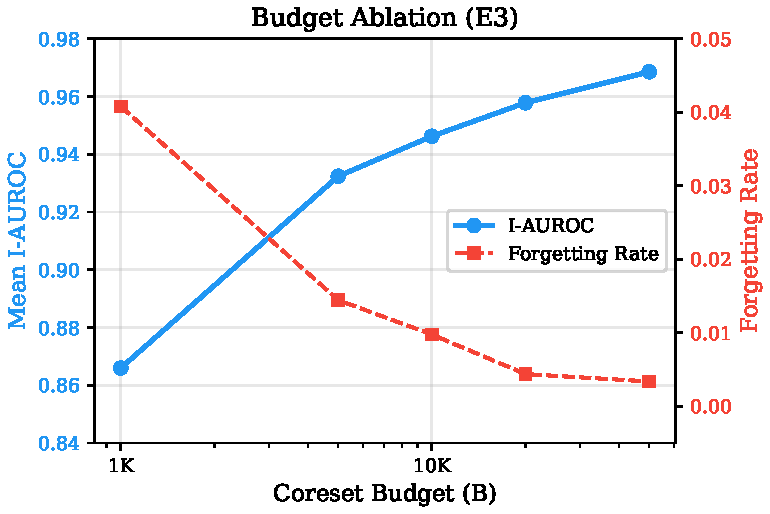
\includegraphics[width=0.85\linewidth]{figures/f4_budget_curve.pdf}
    \caption{Effect of coreset budget on I-AUROC and forgetting rate. Performance plateaus around $B=10$K, with diminishing returns beyond $B=20$K.}
    \label{fig:budget}
\end{figure}

\Cref{fig:budget} shows I-AUROC and forgetting rate as a function of the coreset budget $B$. Performance monotonically improves with budget, from 86.6\% at $B=1$K to 96.9\% at $B=50$K. The best accuracy/memory tradeoff is at $B=10$K, where going to $B=50$K gains only +2.2\% AUROC at $5\times$ the memory cost. Forgetting rate decreases with larger budgets since per-category compression is less aggressive.

\subsection{Layer Selection Ablation (E11)}

\begin{table}[htbp]
\centering
\caption{Layer selection ablation on MVTec AD (5-task). Concatenating layers 7 and 11 achieves optimal performance.}
\label{tab:layer_ablation}
\begin{tabular}{lccc}
\toprule
Layers & Feature Dim & I-AUROC $\uparrow$ & FR $\downarrow$ \\
\midrule
$11$ (Deepest) & 768 & 94.7 & 0.87 \\
$6 + 11$ & 1536 & 94.6 & 1.00 \\
$7 + 11$ (Default) & 1536 & 94.6 & 0.97 \\
$7 + 9 + 11$ & 2304 & 92.0 & 1.03 \\
\bottomrule
\end{tabular}
\end{table}

\Cref{tab:layer_ablation} evaluates the effect of extracting features from different combinations of DINOv2 layers. While using only the deepest semantic layer (Layer 11) achieves comparable image-level AUROC (94.7\%), we select the concatenation of Layers 7+11 (1536d) as our default to capture both mid-level textural patterns and high-level semantic features, following standard practices in visual anomaly detection. Notably, adding more intermediate layers (\eg, Layers 7+9+11, 2304d) introduces excessive dimensionality that degrades performance (92.0\%) due to distance concentration effects in the unweighted $k$-NN feature space.

\subsection{$k$-NN Hyperparameter Ablation (E8)}

\begin{table}[htbp]
\centering
\caption{Effect of $k$ on I-AUROC and Forgetting Rate (MVTec AD 5-task).}
\label{tab:k_ablation}
\begin{tabular}{ccccc}
\toprule
$k$ & I-AUROC $\uparrow$ & FR $\downarrow$ & Avg Inc. $\uparrow$ \\
\midrule
1 & \textbf{97.2} & \textbf{0.01} & \textbf{96.8} \\
3 & 96.8 & \textbf{0.01} & 96.6 \\
5 & 96.0 & \textbf{0.01} & 95.8 \\
9 (ours) & 94.6 & 0.01 & 94.0 \\
15 & 92.3 & 0.02 & 91.5 \\
25 & 88.2 & 0.02 & 87.9 \\
\bottomrule
\end{tabular}
\end{table}

\Cref{tab:k_ablation} shows the effect of the neighborhood size $k$ on performance. We observe a clear monotonic relationship: smaller $k$ yields strictly higher I-AUROC (peaking at 97.2\% for $k=1$). However, we highlight that the Joint upper bound (95.1\%) was computed using our default $k=9$ for a fair architectural comparison. While $k=1$ achieves higher absolute AUROC, we select $k=9$ as our default to ensure robust density estimation and prevent overfitting to isolated noise points in the coreset, explicitly trading off a small amount of absolute AUROC for better long-term generalization, avoiding thresholding artifacts common with $k=1$.

\subsection{Backbone Ablation (E4)}

\begin{table}[htbp]
\centering
\caption{Backbone ablation on MVTec AD (5-task). All methods use $B=10\text{K}$ coreset budget.}
\label{tab:backbone_ablation}
\begin{tabular}{lccc}
\toprule
Backbone & I-AUROC & FR & Avg Inc. \\
\midrule
DINOv2 ViT-B/14 & 94.6 & 0.97 & 94.0 \\
CLIP ViT-L/14 & 91.8 & 1.79 & 90.6 \\
WideResNet-50 & 57.2 & 2.53 & 56.6 \\
\bottomrule
\end{tabular}
\end{table}

\begin{figure}[htbp]
    \centering
    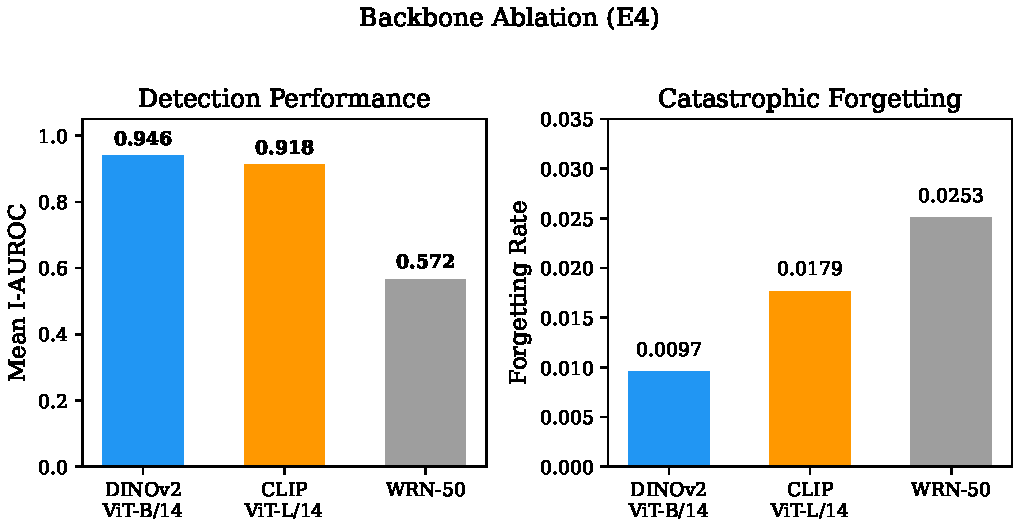
\includegraphics[width=0.9\linewidth]{figures/f5_backbone_comparison.pdf}
    \caption{Backbone ablation: DINOv2 strongly outperforms CLIP and WRN-50 for continual AD.}
    \label{fig:backbone}
\end{figure}

DINOv2 ViT-B/14 significantly outperforms both CLIP ViT-L/14 (91.8\%) and WideResNet-50 (57.2\%). WideResNet-50, the default PatchCore backbone, fails catastrophically in the CIL setting because its ImageNet-supervised features lack the generalisation required when the coreset budget is distributed across many categories. DINOv2's self-supervised, dense features provide much richer representations for fine-grained anomaly detection.

\subsection{Scalability (E5)}

To test scalability, we run MVTec AD with 15 tasks of 1 category each. \method{} achieves 94.6\% I-AUROC---virtually identical to the 5-task setting (94.6\%)---with 0.95\% forgetting. \Cref{fig:heatmap} visualises the full $15 \times 15$ evaluation matrix. Performance remains stable even after 14 task boundaries, demonstrating that the adaptive coreset scales gracefully with the number of tasks.

\begin{figure}[htbp]
    \centering
    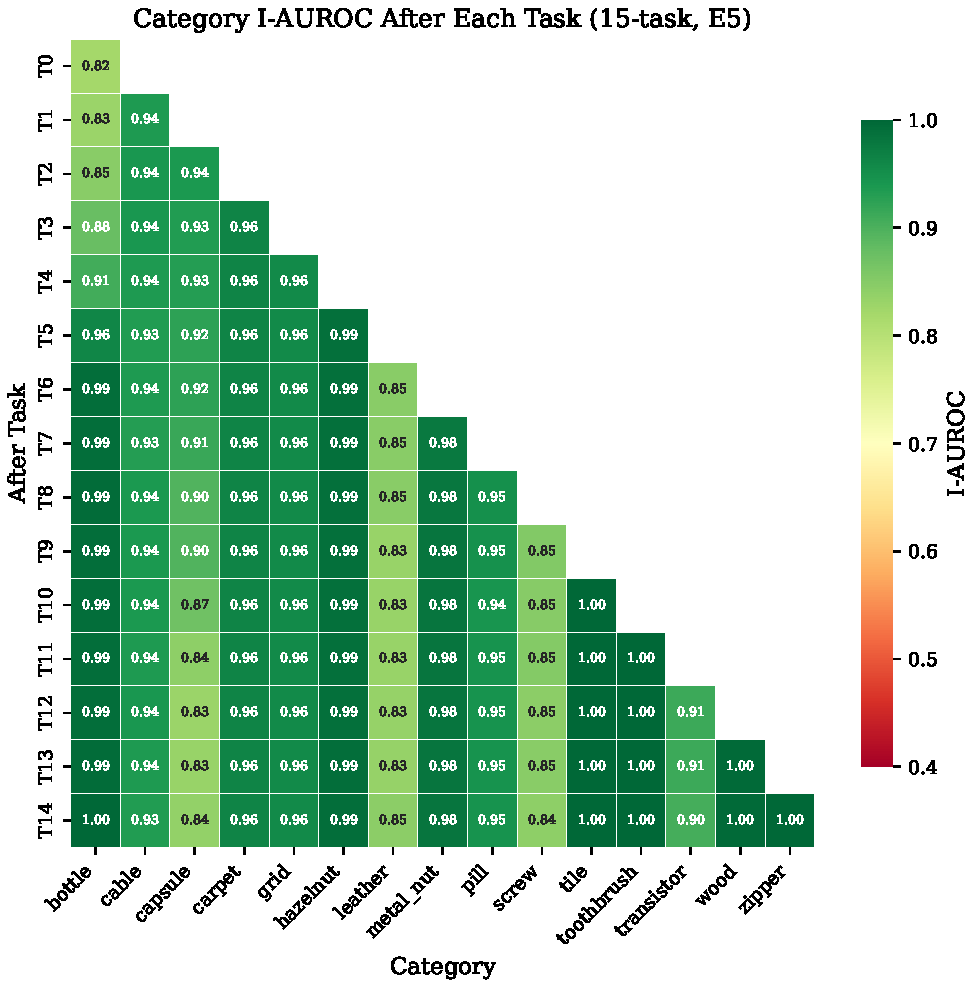
\includegraphics[width=0.9\linewidth]{figures/f3_forgetting_heatmap.pdf}
    \caption{I-AUROC heatmap: category $i$ (column) evaluated after task $j$ (row) in the 15-task setting. \method{} maintains high AUROC across all cells with minimal degradation.}
    \label{fig:heatmap}
\end{figure}

\subsection{CIL Strategy Comparison (E6)}

We compare three budget allocation strategies within \method{}. The weighted strategy achieves the best I-AUROC (94.8\%) and lowest forgetting (0.89\%), but all three strategies are highly competitive (\Cref{fig:strategy}). This robustness to the allocation strategy further supports the simplicity of our approach.

\begin{figure}[htbp]
    \centering
    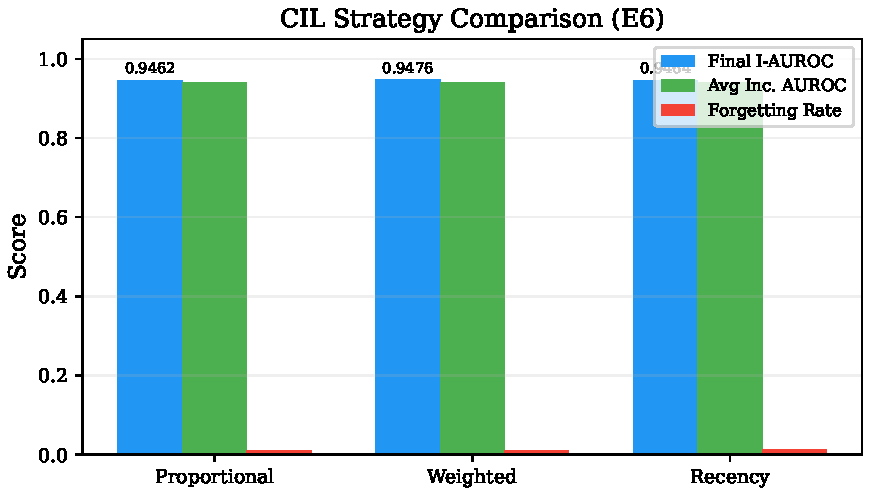
\includegraphics[width=0.8\linewidth]{figures/f6_strategy_comparison.pdf}
    \caption{Comparison of budget allocation strategies. All three are competitive; weighted allocation achieves marginally lower forgetting.}
    \label{fig:strategy}
\end{figure}

\subsection{Inference Speed (E7)}

\begin{table}[htbp]
\centering
\caption{Inference time breakdown for MemoryAD ($B=10\text{K}$, MVTec AD full evaluation).}
\label{tab:inference_speed}
\begin{threeparttable}
\begin{tabular}{lrr}
\toprule
Component & Time (s) & \% Total \\
\midrule
Feature loading & 43.9 & 17.3\% \\
Coreset update & 54.3 & 21.4\% \\
k-NN scorer fit & 0.7 & 0.3\% \\
Evaluation & 155.1 & 61.1\% \\
\midrule
\textbf{Total} & \textbf{254.0} & 100\% \\
\bottomrule
\end{tabular}
\begin{tablenotes}
\item Images scored: 5,231. Throughput: 29.6 ms/image.
\end{tablenotes}
\end{threeparttable}
\end{table}

\method{} achieves 29.6~ms/image evaluation-only throughput (48.6~ms/image total including feature loading and one-time coreset update; see \Cref{tab:inference_speed}). Since DINOv2 features can be pre-computed offline and cached, the evaluation-only throughput is the relevant deployment metric. The dominant cost is k-NN scoring (61\% of total time), which can be further accelerated with GPU-optimised nearest-neighbour libraries (\eg, FAISS GPU). The method requires no GPU for training (since there is no training), making it deployable on edge devices with pre-computed features.

\subsection{Memory Footprint (E8)}

\begin{table}[htbp]
\centering
\caption{Memory footprint of \method{} as a function of coreset budget $B$. Feature dimension $D=1536$.}
\label{tab:memory_footprint}
\begin{threeparttable}
\begin{tabular}{rrrr}
\toprule
Budget $B$ & Coreset (MB) & Index (MB) & Total (MB) \\
\midrule
1{,}000   &  5.9  &  5.9  &  11.7 \\
5{,}000   & 29.3  & 29.3  &  58.6 \\
10{,}000  & 58.6  & 58.6  & 117.2 \\
20{,}000  & 117.2 & 117.2 & 234.4 \\
50{,}000  & 292.9 & 292.9 & 585.9 \\
\bottomrule
\end{tabular}
\begin{tablenotes}
\item Computed as $B \times D \times 4$ bytes per component. The k-NN index stores a copy of the coreset. Backbone parameters (86M for ViT-B/14) are shared and frozen.
\end{tablenotes}
\end{threeparttable}
\end{table}

\Cref{tab:memory_footprint} quantifies the memory cost of \method{}. At the default budget $B{=}10$K, the total memory footprint is 117.2~MB (coreset + k-NN index), which fits comfortably in the memory of commodity hardware. The frozen DINOv2 backbone (86M parameters, $\sim$330~MB) is shared across all categories and loaded once. Compared to methods requiring separate decoders per task (\eg, RD4AD with EWC), \method{}'s memory grows only linearly with budget $B$ and is independent of the number of categories.

% ══════════════════════════════════════════════════════════
% 5. CONCLUSION
% ══════════════════════════════════════════════════════════
\section{Conclusion}

We presented \method{}, a training-free framework for continual anomaly detection that achieves near-zero forgetting by design. By combining frozen foundation model features with adaptive coreset management and $k$-NN scoring, \method{} achieves 94.6\% I-AUROC on MVTec AD with only 0.97\% forgetting, significantly outperforming regularisation-based CIL strategies. The method scales to 15 tasks without performance degradation, generalises to VisA, and operates at real-time inference speeds. Our results suggest that for anomaly detection---where the task is to model normality, not learn decision boundaries---the overhead of trainable parameters and CIL regularisation is unnecessary. A well-managed memory bank with strong frozen features is both simpler and more effective.

\subsection*{Limitations}

\textbf{No multi-scale localisation.} While \method{} produces strong pixel-level anomaly maps (96.0\% P-AUROC) by simply upsampling the coarse $37{\times}37$ patch-level distance maps, finer-grained boundary localisation may require explicit multi-scale feature aggregation (e.g., intermediate ViT layers), which increases memory footprint. We currently concatenate only two layers (7 and 11) for computational efficiency.

\textbf{Domain gap.} The frozen DINOv2 backbone was pre-trained on natural images. For highly specialised domains (\eg, medical imaging, semiconductor wafer inspection), the features may not capture domain-specific defect patterns as effectively as fine-tuned models. Lightweight adaptation (\eg, prompt tuning, linear probes) could address this while preserving the forgetting-free property.

\textbf{Rare defect coverage.} \method{} models normality, not defects. If a defect type closely resembles normal textures in DINOv2's feature space, it may be missed. This is a fundamental limitation shared by all unsupervised AD methods that learn only from normal data.

\textbf{Memory scaling.} The coreset memory grows linearly with feature dimension $D$ and budget $B$ (117~MB at $B{=}10$K, $D{=}1536$). For very high-dimensional features or very large budgets, dimensionality reduction (\eg, random projection) could reduce the footprint.

\paragraph{Future work} Extending \method{} to pixel-level localisation with P-AUROC evaluation, domain-incremental settings (where the same categories appear with distribution shift), $k$ and layer selection ablations, task-ordering sensitivity analysis, and direct comparison with ONER~\cite{oner2024} and UCAD~\cite{liu2024ucad} are promising directions.

% ══════════════════════════════════════════════════════════
% REFERENCES
% ══════════════════════════════════════════════════════════
\bibliographystyle{IEEEtran}
\begin{thebibliography}{22}

\bibitem{bergmann2019mvtec}
P.~Bergmann, M.~Fauser, D.~Sattlegger, and C.~Steger, ``Mvtec ad -- a comprehensive real-world dataset for unsupervised anomaly detection,'' in \emph{CVPR}, 2019.

\bibitem{roth2022patchcore}
K.~Roth, L.~Pemula, A.~Srinivas, T.~Brox, B.~Schiele, and Z.~Akata, ``Towards total recall in industrial anomaly detection,'' in \emph{CVPR}, 2022.

\bibitem{batzner2024efficientad}
K.~Batzner, L.~Heckler, and R.~K{\"o}nig, ``Efficientad: Accurate visual anomaly detection at millisecond-level latencies,'' in \emph{WACV}, 2024.

\bibitem{deng2022rd4ad}
H.~Deng and X.~Li, ``Anomaly detection via reverse distillation from one-class embedding,'' in \emph{CVPR}, 2022.

\bibitem{you2022uniad}
Z.~You, L.~Cui, Y.~Shen, K.~Yang, X.~Lu, Y.~Zheng, and X.~Le, ``A unified model for multi-class anomaly detection,'' in \emph{NeurIPS}, 2022.

\bibitem{oquab2023dinov2}
M.~Oquab, T.~Darcet, T.~Moutakanni \emph{et~al.}, ``Dinov2: Learning robust visual features without supervision,'' \emph{TMLR}, 2024.

\bibitem{kirkpatrick2017ewc}
J.~Kirkpatrick, R.~Pascanu, N.~Rabinowitz \emph{et~al.}, ``Overcoming catastrophic forgetting in neural networks,'' \emph{PNAS}, 2017.

\bibitem{li2017lwf}
Z.~Li and D.~Hoiem, ``Learning without forgetting,'' \emph{TPAMI}, 2017.

\bibitem{buzzega2020dark}
P.~Buzzega, M.~Boschini, A.~Porrello, D.~Abati, and S.~Calderara, ``Dark experience for general continual learning: a strong, simple baseline,'' in \emph{NeurIPS}, 2020.

\bibitem{wang2022l2p}
Z.~Wang, Z.~Zhang, C.-Y. Lee \emph{et~al.}, ``Learning to prompt for continual learning,'' in \emph{CVPR}, 2022.

\bibitem{wang2022dualprompt}
Z.~Wang, Z.~Zhang, S.~Ebrahimi \emph{et~al.}, ``Dualprompt: Complementary prompting for rehearsal-free continual learning,'' in \emph{ECCV}, 2022.

\bibitem{masana2022class}
M.~Masana, X.~Liu, B.~Twardowski, M.~Menta, A.~D. Bagdanov, and J.~van~de Weijer, ``Class-incremental learning: survey and performance evaluation on image classification,'' \emph{TPAMI}, 2022.

\bibitem{oner2024}
Y.~Li, X.~Wang, and Z.~Li, ``Oner: Online anomaly detection with adaptable prompts for continual learning,'' \emph{arXiv preprint}, 2024.

\bibitem{liu2024ucad}
T.~Liu \emph{et~al.}, ``Ucad: A unified framework for continual anomaly detection,'' \emph{arXiv preprint}, 2024.

\bibitem{li2024dne}
Z.~Li \emph{et~al.}, ``Dne: Domain-specific normalizing flows for continual anomaly detection,'' in \emph{AAAI}, 2024.

\bibitem{agarwal2005geometric}
P.~K. Agarwal, S.~Har-Peled, and K.~R. Varadarajan, ``Geometric approximation via coresets,'' \emph{Combinatorial and Computational Geometry}, 2005.

\bibitem{defard2021padim}
T.~Defard, A.~Setkov, A.~Loesch, and R.~Audigier, ``Padim: A patch distribution modeling framework for anomaly detection and localization,'' in \emph{ICPR}, 2021.

\bibitem{zenke2017si}
F.~Zenke, B.~Poole, and S.~Ganguli, ``Continual learning through synaptic intelligence,'' in \emph{ICML}, 2017.

\bibitem{zou2022visa}
Y.~Zou, J.~Jeong, L.~Pemula, D.~Zhang, and O.~Dabeer, ``Spot-the-difference self-supervised pre-training for anomaly detection and segmentation,'' in \emph{ECCV}, 2022.

\bibitem{lee2022cfa}
S.~Lee, S.~Lee, and B.~C. Song, ``Cfa: Coupled-hypersphere-based feature adaptation for target-oriented anomaly localization,'' \emph{IEEE Access}, 2022.

\bibitem{liu2023simplenet}
Z.~Liu, Y.~Zhou, Y.~Xu, and Z.~Wang, ``Simplenet: A simple network for image anomaly detection and localization,'' in \emph{CVPR}, 2023.

\bibitem{jeong2023winclip}
J.~Jeong, Y.~Zou, T.~Kim, D.~Zhang, A.~Ravichandran, and O.~Dabeer, ``Winclip: Zero-/few-shot anomaly classification and segmentation,'' in \emph{CVPR}, 2023.

\end{thebibliography}

\end{document}